\documentclass{standalone}
\usepackage{tikz}
\usetikzlibrary{patterns, positioning}

\begin{document}
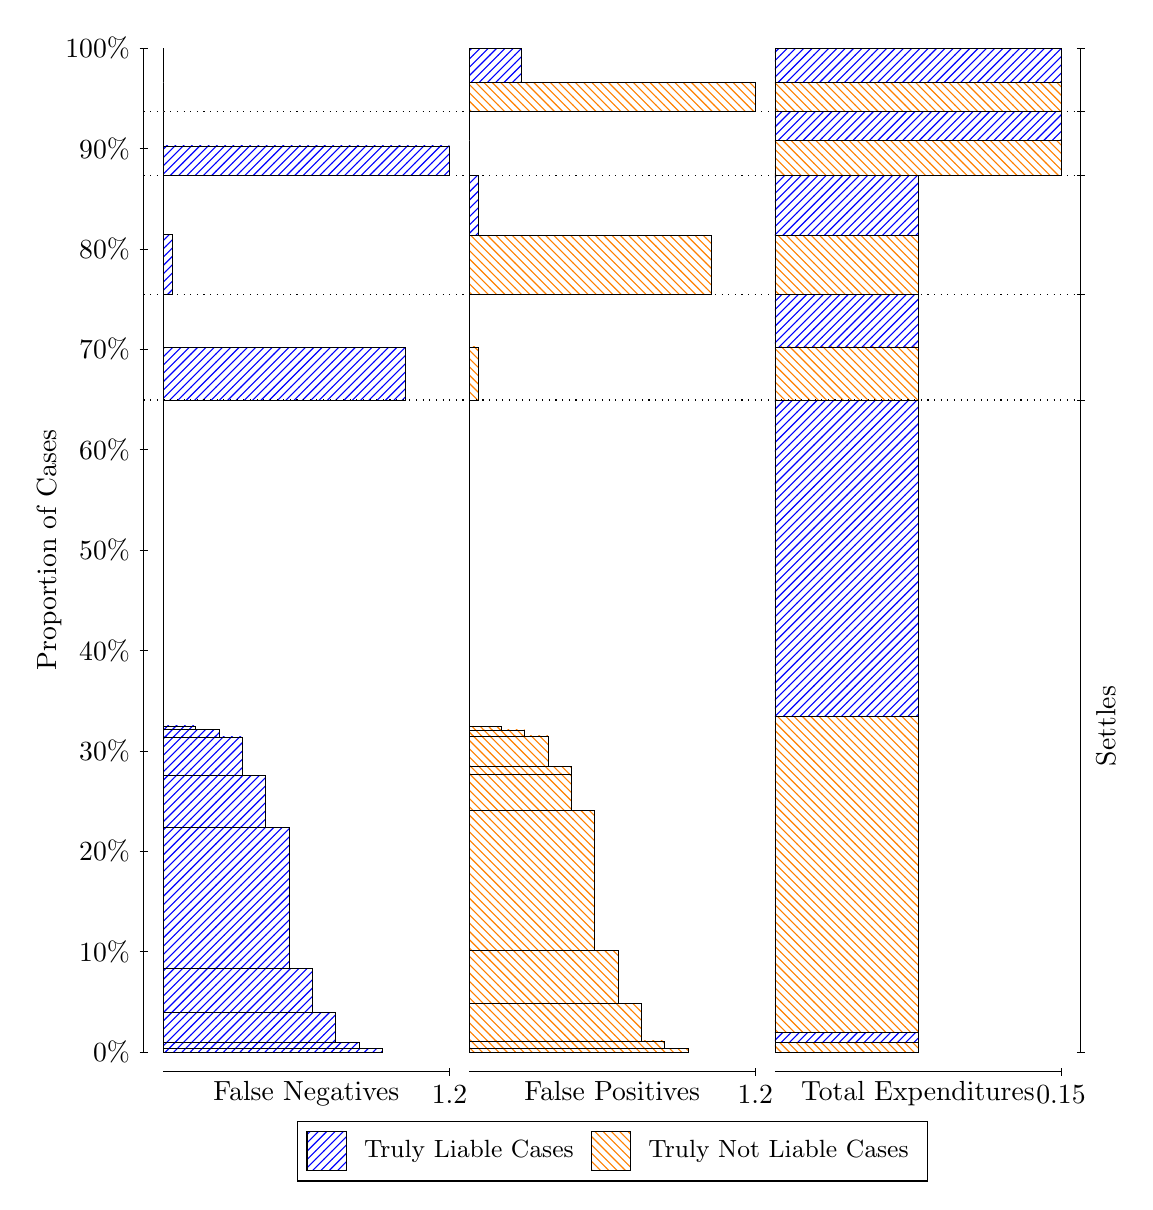
\begin{tikzpicture}
\draw[black, very thin] (1.5,1.75) -- (1.5,14.5);
\node[rotate=90, anchor=center] at (0.3, 8.125) {Proportion of Cases};
\draw[black, very thin] (1.45,1.75) -- (1.55,1.75);
\node[anchor=east] at (1.45, 1.75) {0\%};
\draw[black, very thin] (1.45,3.025) -- (1.55,3.025);
\node[anchor=east] at (1.45, 3.025) {10\%};
\draw[black, very thin] (1.45,4.3) -- (1.55,4.3);
\node[anchor=east] at (1.45, 4.3) {20\%};
\draw[black, very thin] (1.45,5.575) -- (1.55,5.575);
\node[anchor=east] at (1.45, 5.575) {30\%};
\draw[black, very thin] (1.45,6.85) -- (1.55,6.85);
\node[anchor=east] at (1.45, 6.85) {40\%};
\draw[black, very thin] (1.45,8.125) -- (1.55,8.125);
\node[anchor=east] at (1.45, 8.125) {50\%};
\draw[black, very thin] (1.45,9.4) -- (1.55,9.4);
\node[anchor=east] at (1.45, 9.4) {60\%};
\draw[black, very thin] (1.45,10.675) -- (1.55,10.675);
\node[anchor=east] at (1.45, 10.675) {70\%};
\draw[black, very thin] (1.45,11.95) -- (1.55,11.95);
\node[anchor=east] at (1.45, 11.95) {80\%};
\draw[black, very thin] (1.45,13.225) -- (1.55,13.225);
\node[anchor=east] at (1.45, 13.225) {90\%};
\draw[black, very thin] (1.45,14.5) -- (1.55,14.5);
\node[anchor=east] at (1.45, 14.5) {100\%};

\draw[black, very thin] (13.4,1.75) -- (13.4,14.5);
\draw[black, very thin] (13.35,1.75) -- (13.45,1.75);
\node[anchor=west] at (13.35, 1.75) {};
\draw[black, very thin] (13.35,10.03) -- (13.45,10.03);
\node[anchor=west] at (13.35, 10.03) {};
\draw[black, very thin] (13.35,11.369) -- (13.45,11.369);
\node[anchor=west] at (13.35, 11.369) {};
\draw[black, very thin] (13.35,12.886) -- (13.45,12.886);
\node[anchor=west] at (13.35, 12.886) {};
\draw[black, very thin] (13.35,13.693) -- (13.45,13.693);
\node[anchor=west] at (13.35, 13.693) {};
\draw[black, very thin] (13.35,14.5) -- (13.45,14.5);
\node[anchor=west] at (13.35, 14.5) {};

\draw[black, very thin, pattern color=blue, pattern=north east lines] (1.75,1.75) rectangle (4.5306,1.7953);
\draw[black, very thin, pattern color=blue, pattern=north east lines] (1.75,1.7953) rectangle (4.234,1.8713);
\draw[black, very thin, pattern color=blue, pattern=north east lines] (1.75,1.8713) rectangle (3.9374,2.2571);
\draw[black, very thin, pattern color=blue, pattern=north east lines] (1.75,2.2571) rectangle (3.6408,2.8073);
\draw[black, very thin, pattern color=blue, pattern=north east lines] (1.75,2.8073) rectangle (3.3442,4.6008);
\draw[black, very thin, pattern color=blue, pattern=north east lines] (1.75,4.6008) rectangle (3.0476,5.266);
\draw[black, very thin, pattern color=blue, pattern=north east lines] (1.75,5.266) rectangle (2.751,5.7512);
\draw[black, very thin, pattern color=blue, pattern=north east lines] (1.75,5.7512) rectangle (2.4544,5.8503);
\draw[black, very thin, pattern color=blue, pattern=north east lines] (1.75,5.8503) rectangle (2.1578,5.8924);
\draw[black, very thin, pattern color=orange, pattern=north west lines] (1.75,5.8924) rectangle (1.75,10.03);
\draw[black, very thin, pattern color=blue, pattern=north east lines] (1.75,10.03) rectangle (4.8272,10.695);
\draw[black, very thin, pattern color=orange, pattern=north west lines] (1.75,10.695) rectangle (1.75,11.369);
\draw[black, very thin, pattern color=blue, pattern=north east lines] (1.75,11.369) rectangle (1.8612,12.131);
\draw[black, very thin, pattern color=orange, pattern=north west lines] (1.75,12.131) rectangle (1.75,12.886);
\draw[black, very thin, pattern color=blue, pattern=north east lines] (1.75,12.886) rectangle (5.3833,13.256);
\draw[black, very thin, pattern color=orange, pattern=north west lines] (1.75,13.256) rectangle (1.75,13.693);
\draw[black, very thin, pattern color=orange, pattern=north west lines] (1.75,13.693) rectangle (1.75,14.064);
\draw[black, very thin, pattern color=blue, pattern=north east lines] (1.75,14.064) rectangle (1.75,14.5);
\draw[black, very thin, pattern color=orange, pattern=north west lines] (5.6333,1.75) rectangle (8.4139,1.792);
\draw[black, very thin, pattern color=orange, pattern=north west lines] (5.6333,1.792) rectangle (8.1173,1.8895);
\draw[black, very thin, pattern color=orange, pattern=north west lines] (5.6333,1.8895) rectangle (7.8207,2.3706);
\draw[black, very thin, pattern color=orange, pattern=north west lines] (5.6333,2.3706) rectangle (7.5241,3.0358);
\draw[black, very thin, pattern color=orange, pattern=north west lines] (5.6333,3.0358) rectangle (7.2276,4.8208);
\draw[black, very thin, pattern color=orange, pattern=north west lines] (5.6333,4.8208) rectangle (6.931,5.282);
\draw[black, very thin, pattern color=orange, pattern=north west lines] (5.6333,5.282) rectangle (6.931,5.3731);
\draw[black, very thin, pattern color=orange, pattern=north west lines] (5.6333,5.3731) rectangle (6.6344,5.7635);
\draw[black, very thin, pattern color=orange, pattern=north west lines] (5.6333,5.7635) rectangle (6.3378,5.8411);
\draw[black, very thin, pattern color=orange, pattern=north west lines] (5.6333,5.8411) rectangle (6.0412,5.8881);
\draw[black, very thin, pattern color=blue, pattern=north east lines] (5.6333,5.8881) rectangle (5.6333,10.03);
\draw[black, very thin, pattern color=orange, pattern=north west lines] (5.6333,10.03) rectangle (5.7446,10.705);
\draw[black, very thin, pattern color=blue, pattern=north east lines] (5.6333,10.705) rectangle (5.6333,11.369);
\draw[black, very thin, pattern color=orange, pattern=north west lines] (5.6333,11.369) rectangle (8.7105,12.124);
\draw[black, very thin, pattern color=blue, pattern=north east lines] (5.6333,12.124) rectangle (5.7446,12.886);
\draw[black, very thin, pattern color=orange, pattern=north west lines] (5.6333,12.886) rectangle (5.6333,13.323);
\draw[black, very thin, pattern color=blue, pattern=north east lines] (5.6333,13.323) rectangle (5.6333,13.693);
\draw[black, very thin, pattern color=orange, pattern=north west lines] (5.6333,13.693) rectangle (9.2667,14.064);
\draw[black, very thin, pattern color=blue, pattern=north east lines] (5.6333,14.064) rectangle (6.3007,14.5);
\draw[black, very thin, pattern color=orange, pattern=north west lines] (9.5167,1.75) rectangle (11.333,1.8746);
\draw[black, very thin, pattern color=blue, pattern=north east lines] (9.5167,1.8746) rectangle (11.333,1.9959);
\draw[black, very thin, pattern color=orange, pattern=north west lines] (9.5167,1.9959) rectangle (11.333,6.0094);
\draw[black, very thin, pattern color=blue, pattern=north east lines] (9.5167,6.0094) rectangle (11.333,10.03);
\draw[black, very thin, pattern color=orange, pattern=north west lines] (9.5167,10.03) rectangle (11.333,10.705);
\draw[black, very thin, pattern color=blue, pattern=north east lines] (9.5167,10.705) rectangle (11.333,11.369);
\draw[black, very thin, pattern color=orange, pattern=north west lines] (9.5167,11.369) rectangle (11.333,12.124);
\draw[black, very thin, pattern color=blue, pattern=north east lines] (9.5167,12.124) rectangle (11.333,12.886);
\draw[black, very thin, pattern color=orange, pattern=north west lines] (9.5167,12.886) rectangle (13.15,13.323);
\draw[black, very thin, pattern color=blue, pattern=north east lines] (9.5167,13.323) rectangle (13.15,13.693);
\draw[black, very thin, pattern color=orange, pattern=north west lines] (9.5167,13.693) rectangle (13.15,14.064);
\draw[black, very thin, pattern color=blue, pattern=north east lines] (9.5167,14.064) rectangle (13.15,14.5);
\draw[black, dotted] (1.5,10.03) -- (13.4,10.03);
\draw[black, dotted] (1.5,11.369) -- (13.4,11.369);
\draw[black, dotted] (1.5,12.886) -- (13.4,12.886);
\draw[black, dotted] (1.5,13.693) -- (13.4,13.693);
\draw[black, very thin] (1.75,1.5) -- (5.3833,1.5);
\node[anchor=north] at (3.5667, 1.5) {False Negatives};
\draw[black, very thin] (5.3833,1.45) -- (5.3833,1.55);
\node[anchor=north] at (5.3833, 1.45) {1.2};

\draw[black, very thin] (5.6333,1.5) -- (9.2667,1.5);
\node[anchor=north] at (7.45, 1.5) {False Positives};
\draw[black, very thin] (9.2667,1.45) -- (9.2667,1.55);
\node[anchor=north] at (9.2667, 1.45) {1.2};

\draw[black, very thin] (9.5167,1.5) -- (13.15,1.5);
\node[anchor=north] at (11.333, 1.5) {Total Expenditures};
\draw[black, very thin] (13.15,1.45) -- (13.15,1.55);
\node[anchor=north] at (13.15, 1.45) {0.15};

\node[black, centered, rotate=90] at (13.72, 5.8902) {Settles};





\draw (7.449999999999999,1.5) node[draw=none] (baseCoordinate) {};
\begin{scope}[align=center]
        \matrix[scale=0.5, draw=black, below=0.5cm of baseCoordinate, nodes={draw}, column sep=0.1cm]{
            \node[rectangle, draw, minimum width=0.5cm, minimum height=0.5cm, pattern=north east lines, pattern color=blue] {}; &
            \node[draw=none, font=\small] (B) {Truly Liable Cases}; &
            \node[rectangle, draw, minimum width=0.5cm, minimum height=0.5cm, pattern=north west lines, pattern color=orange] {}; &
            \node[draw=none, font=\small] (B) {Truly Not Liable Cases}; \\
            };
\end{scope}

\end{tikzpicture}
\end{document}